%authentication use case

\subsubsection{Authentication}
UPRM works with sensitive and personal data therefore security plays a massive role in UPRM.
Users will be required to login with a username, password and one-time generated password. UPRM will therefore have build-in two step authentication. \\ \\
A user will be authenticated against LDAP with their username and password. Once LDAP authentication is successful a one-time pin will be generated for the user.\\ \\
Access rights and privileges will be set by an admin user. The admin user will have full access rights and privileges to UPRM.\\ \\
\textbf{Use Cases:}
\begin{itemize}
	\item Register New User
	\item Login
	\item Logout \\
\end{itemize}
\textbf{Authentication Use Case Overview Diagram:}\\
\centerline{\fbox{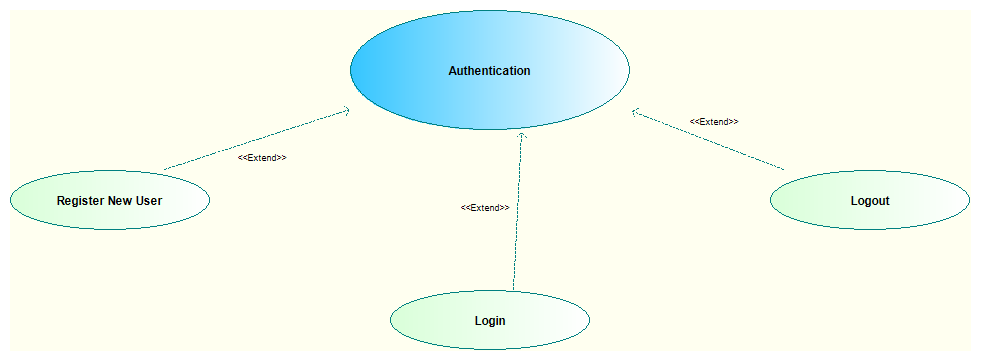
\includegraphics[width=\linewidth]{auth/OverviewAuthUseCase}}}


